\documentclass[12pt]{article}
\usepackage{fullpage}
\usepackage{graphicx}
\usepackage{url}
\title{Cryptography Coursework}
\author{Jordan Milton - jksm1g10}

\begin{document}
\maketitle

\section{Question 1: Elliptic Curves}

The first part of this question involves working out the order of a group for a given elliptic curve over a field. The curve and field assigned to me was $y^2 = x^3 + 8x + 4$ over the field $Z_{17}$. This was calculated by finding every point on the curve (shown in table \ref{table:elems}), being careful to not forget the point at infinity. In order to do this I wrote a program in c which prints the order and elements for a given group. The order is 21.

\begin{table}[h!]
\label{table:elems}
\centering
\begin{tabular}{| c | c |}
 \hline
\textbf{X} & \textbf{Y} \\ \hline
0 & 2 \\ \hline
0 & 15 \\ \hline
1 & 8 \\ \hline
1 & 9 \\ \hline
3 & 2 \\ \hline
3 & 15 \\ \hline
4 & 7 \\ \hline
4 & 10 \\ \hline
5 & 4 \\ \hline
5 & 13 \\ \hline
6 & 8 \\ \hline
6 & 9 \\ \hline
8 & 6 \\ \hline
8 & 11 \\ \hline
10 & 8 \\ \hline
10 & 9 \\ \hline
12 & 3 \\ \hline
12 & 14 \\ \hline
14 & 2 \\ \hline
14 & 15 \\ \hline
\end{tabular}
\caption{Table of elements in the group (not including the point at infinity)}
\end{table}

Next, I was tasked with determing whether the group I was given was cyclic. The group's prime factors are $3 * 7$. As neither are repeated, this means that the group must be $C_{21}$.

The last task is to use this elliptic curve to construct a secure cipher. One way to do this would be by using Diffie-Hellman key exchange to create a shared secret. This secret can then be used to cipher the text, and the only person who can also decrypt is the person with whom the secret was created.

In order to do this, both parties must first agree on an elliptic curve and a generator. Then each participant selects a large secret number, and raises the generator to that power. The new group members are then exchanged, and each party raises the recieved member by their secret number. So, if the generator is $g$ and the secret numbers are $a$ and $b$, the final shared secret equals $(g^a)^b$ which is identical to $(g^b)^a$. The reason this works is because calculating the discrete logarithm is much harder than raising to a power. That is, given $g, g^i$ it is very difficult to calculate $i$ if $i$ is large.

Finally, we still need to actually create the cipher. I used cypher block chaining. While it isn't the most secure system, it is quite easy to implement. I make use of 2 keys created via Diffy-Hellman, the first is used as the initialisation vector and the second is combined with the text with exclusive OR. The group members in their coordinate form aren't appropriate, so the $X$ coordinate is used. The output of a simulated secure transmission is shown in figure \ref{fig:output}. The two lines between the message (A little knowledge is a dangerous thing) are the printed form of the enciphered text.

\begin{figure}[!h]
\label{fig:output}
\centering
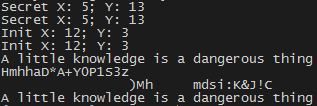
\includegraphics[keepaspectratio=true]{qOneOutput}
\caption{Output from faked transmission using an elliptic curve cipher}
\end{figure}

\section{Question 2: Decrypt a message}

This question involved decrypting a paragraph of cipher text. The text has the right features to suggest confusion without diffusion, as in the letters have been changed but not their positions. The spaces in the text look like sensible places for there to be spaces, which is what implies the lack of character movement. As this question was set for a coursework, it had to be a cipher that could merit $12.5\%$ of a modules total mark. This immediately rules out a straight caesar cipher or a substitution cipher. The next most obvious choice was a Vigen\`ere cipher.

In order to confirm it was indeed a Vigen\`ere cipher, I wrote some code that calculated the index of coincidence (IoC) at a given step (if the key was two characters long, the step would be 2). I then wrapped it with a function that would test the IoC for every step between two and twelve inclusive, and then returned the results highest IoC first. The top three results were six, three and nine. All of which had an index of coincidence close to that of natural English (about 1.7\footnote{\url{http://en.wikipedia.org/wiki/Index_of_coincidence}}), which made it incredibly likely that a Vigen\`ere cipher was used. Those three have very similar ICs, but as three was the common factor I chose to test that first.

In order to actually get the original text back, I had to split the text into three columns and then solve their individual caeser shifts. As the key size was small, it was possible to brute force the solution once I had the columns. I wrote code that tried every possible combination of caeser shifts across all three columns, and then ran a dictionary\footnote{dictionary provided by \url{http://en-gb.pyxidium.co.uk/dictionary/OOo.php}} check against the possible rebuilds to get a shortlist of candidates. As it happened, there was only one correct solution as shown in figure \ref{fig:vigoutput}.

\begin{figure}[!h]
\label{fig:vigoutput}
\centering
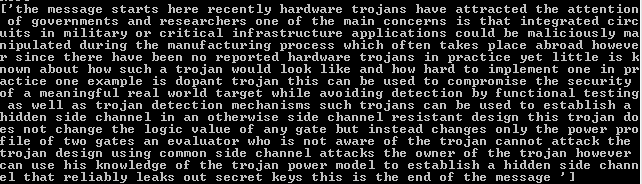
\includegraphics[keepaspectratio=true]{qTwoOutput}
\caption{Sorry for the terrible word wrap}
\end{figure}

\section{Question 3: Decrypt a hex file}

In this question we were supplied a secret.hex file, which contains some encrypted message. We are also given a crib of the intermediary stage (first two characters are "Hg"), and the process used for the second stage of ciphering. The important thing to realise, which took me an alarmingly long time, is that the second stage of the ciphering is the first stage of decrypting.

With that knowledge in hand, getting the first two bytes of the key was trivial. The first two bytes of the cipher XOR'd against the crib would give me the first two bytes of the key. Given the crib that this is coursework, it was probable that this was a repeated key. Indeed, after XORing the original bytes against the repeated key I had an amount of text that looked like a reasonable intermediary step (figure \ref{fig:intermediary}).

\begin{figure}[!h]
\label{fig:intermediary}
\begin{tabular}{|l|}
 \hline
Hgt ltsbuba pm dumt uy hgt lpyh wqpmpxbr sbr tdxyuct lvyhtqv pm hgtl sdd,\\ xbobpib hp tctb hgt aqtshtyh lubry. Yxqtdv sbvpbt igp htddy vpx hgtv gsct\\ hgt sbyitq uy npouba, lsr pq yulwdv luyhsotb. Hgtqt sqt lsbv hgubay hgsh\\ lsot dumt ipqhg gpdruba pb hp sbr yscpxquba. Exh dumt uy xbwqtrukhsedt sbr\\ it sqt pmhtb lvyhtquty tctb hp pxqytdcty. It hgubo yxkktyy, gswwubtyy,\\ gtdwuba phgtqy, pq yxqwsyyuba pxqytdcty iudd lsot dumt ipqhg ducuba, exh\\ it ksb sdisvy et iqpba pq mqxyhqshtr ev tctbhy. Hguy uy s qsbrpl wgqsyt.\\ Wgudpypwgtqy gsct s dph hp ysv sepxh hgt csdxt pm sdd hgtyt hgubay, sbr\\ s duhhdt dtyy hp ysv sepxh pbt pm hgt lpyh csdxsedt hgubay pm sdd: dpct. Yp\\ it ksb et kdtsq tbpxag sepxh igsh uh ltsby mpq dumt hp gsct ltsbuba sbr\\ csdxt, exh igtb it wxh rpib pxq wgudpypwgv eppoy sbr skhxsddv ath pb iuhg\\ ducuba, ltsbuba sbr csdxt ksb et tdxyuct. Ducuba itdd uy lpqt sqh hgsb \\ykutbkt pq wgudpypwgv. Hgtqtmpqt,  hgt pbdv ytbyt it ksb lsot pm hgt urts\\ hgsh dumt gsy ltsbuba uy hgsh hgtqt sqt yplt qtsypby hp duct qshgtq hgsb hp\\ rut, sbr hgpyt qtsypby sqt hp et mpxbr ub hgt ducuba pm dumt uhytdm.\\
\hline
\end{tabular}
\caption{Output halfway through question 3}
\end{figure}

The text has similar features to the one from question 2. The spaces and punctiation look like they are where they should be, which implies confusion without diffusion. As the previous challenge had been a Vigen\`ere cipher, I doubted this was also. A caesar cipher still seemed too simple, and so I decided to try substitution. I attacked this with the aid of an online tool\footnote{\url{http://www.simonsingh.net/The_Black_Chamber/substitutioncrackingtool.html}} that allowed me to try different alphabets one character at a time and see the resulting decrypted text in real time. I starte the attack on "Hgt", which looked like it would be "The". From there I kept completing words that looked right until I had the whole text decrypte (figure \ref{fig:qThreeOut}).

\begin{figure}[!h]
\label{fig:qThreeOut}
\begin{tabular}{|l|}
 \hline
The meaning of life is the most profound and elusive mystery of them all,\\ unknown to even the greatest minds. Surely anyone who tells you they have\\ the answer is joking, mad or simply mistaken. There are many things that\\ make life worth holding on to and savouring. But life is unpredictable and\\ we are often mysteries even to ourselves. We think success, happiness,\\ helping others, or surpassing ourselves will make life worth living, but we\\ can always be wrong or frustrated by events. This is a random phrase.\\ Philosophers have a lot to say about the value of all these things, and a\\ little less to say about one of the most valuable things of all: love. So we\\ can be clear enough about what it means for life to have meaning and\\ value, but when we put down our philosophy books and actually get on with\\ living, meaning and value can be elusive. Living well is more art than\\ science or philosophy. Therefore,  the only sense we can make of the idea\\ that life has meaning is that there are some reasons to live rather than to\\ die, and those reasons are to be found in the living of life itself.\\
\hline
\end{tabular}
\caption{Output halfway through question 3}
\end{figure}

\section{Question 4: The headline puzzles}

For question four we were tasked with solving the headline puzzles:
\begin{enumerate}
\item YNTS QHABT YBK KJVT NR ORLSJN HCTCYA HQYKJV CYOCMBYNT
\item GXRYK SXRKVWNRNIO YJVONHB NH VH KXASH OAXBBJNHB WNHB
\item KSXXMT, FVTS SVJYMBF CFI EI BNSYYC JTMKEID
\item AXITUL PGGTXLW VGA OCXFT AUMCAL VAGH RXDKQPUR PXDM
\item HQUSESTYY TBDSPKTTY YTT ERYHURBRWCVRPW RW JCBRSKJURTWESK DPSRHRTY
\end{enumerate}

According to information I found online\footnote{\url{https://sites.google.com/site/theheadlinepuzzle/help/about-the-headline-puzzle}}, the encryption method used is a substitution cipher. To solve this, I used the same site as I used for question 3\footnote{\url{http://www.simonsingh.net/The_Black_Chamber/substitutioncrackingtool.html}} for the same reasons as I used it for before. Due to the small message size, there weren't enough words to do standard attacks against it (frequency analysis for example). Instead I looked for words in the dictionary that matched the patterns in the cipher\footnote{This tool was used extensively \url{http://design215.com/toolbox/wordpattern.php}}. After selecting likely candidates, I made the required substitutions. This then gave me more information with which to find candidates for other words in the cipher. I repeated this process untill all letters were found. The solutions were:
\begin{enumerate}
\item NTSB URGES NEW WAYS TO COMBAT RISING RUNWAY INCIDENTS
\item DUTCH AUTHORITIES CLOSING IN ON HUMAN SMUGGLING RING
\item DOLLAR, EURO OUTPACE YEN IN CHOPPY TRADING
\item RIPKEN LOOKING FOR QUICK RETURN FROM DISABLED LIST
\item CHRLDLESS EMPLOYEES SEE DISCRIMINATION IN FAMILYFRIENDLY POLICIES
\end{enumerate}

\end{document}
